%&pdflatex
\documentclass{article}
\usepackage[final]{nips_2017}
\usepackage[utf8]{inputenc} % allow utf-8 input
\usepackage[T1]{fontenc}    % use 8-bit T1 fonts
\usepackage{hyperref}       % hyperlinks
\usepackage{url}            % simple URL typesetting
\usepackage{booktabs}       % professional-quality tables
\usepackage{amsfonts}       % blackboard math symbols
\usepackage{nicefrac}       % compact symbols for 1/2, etc.
\usepackage{microtype}      % microtypography
\usepackage{amsmath}
\usepackage{mathtools}
\usepackage{graphicx}
\usepackage{tabu}
\usepackage{mathrsfs}
\usepackage{morefloats}
\usepackage{float}
\usepackage{listings}
\usepackage[usenames,dvipsnames]{xcolor}
\usepackage{commath}
\usepackage{graphicx}
\usepackage{tikz,tikz-3dplot}
\usetikzlibrary{calc}
\usetikzlibrary{intersections}

% Define the coloring for keywords in Julia
\lstdefinelanguage{Julia}%
{morekeywords={abstract,break,case,catch,const,continue,do,else,elseif,%
    end,export,false,for,function,immutable,import,importall,if,in,%
    macro,module,otherwise,quote,return,switch,true,try,type,typealias,%
    using,while},%
  sensitive=true,%
  morecomment=[l]\#,%
  morecomment=[n]{\#=}{=\#},%
  morestring=[s]{"}{"},%
  morestring=[m]{'}{'},%
}[keywords,comments,strings]%

% Set the lstlistings to the Julia color scheme
\lstset{
  basicstyle       = \ttfamily,
  columns          = fullflexible,
  frame            = single,
  breaklines       = true,
  language         = Julia,
  basicstyle       = \ttfamily,
  keywordstyle     = \bfseries\color{blue},
  stringstyle      = \color{magenta},
  commentstyle     = \color{ForestGreen},
  showstringspaces = false,
  numbers          = left,
  xleftmargin      = 2em,
  framexleftmargin = 2em
}

\title{Scale Space Edge Detection}

\author{
  Nick Draper, Jonathan Hayase\\
  Seminar in Differential Geometry\\
  Harvey Mudd College
}

\begin{document}
\maketitle

\begin{abstract}
  Scale space representation is the idea that a two dimensional image can be represented by a collection of smoothed images.
  This paper documents how using such a representation can be useful for detecting edges in an image.
  The scale space allows for a classification of how strong different edges are in the image from very fine to coarse ones. 
\end{abstract}

\section{Edge Detection Background}
Detecting edges in images has long been a problem with many uniques solutions to approach it.
Generally speaking, the majority of algorithms are usually checking the image for some of the following features:

\begin{itemize}
\item large discontinuities in luminance values
\item discontinuities in different object orientations
\item large discontinuities in the intensity gradient
\end{itemize}
\indent Some of the common methods for edge detection include the Sobel, Canny, Prewitt, Roberts, and Fuzzy Logic algorithms.
However, these methods do not yield a lot of information with regards to the strength of the edges detected.
The majority of these algorithms will usually convolve the image with a static matrix to calculate edges and does adapt enough to the image. 

This is why for our edge detection method, we will be using the scale space approach.
The benefit of using a scale space approach for edge detection, is we have the ability to classify the strength of the edges in the image.
This allows for a range of edges from very large immediate changes in intensity to very gradual.

\section{Scale Space and Its Derivatives}
To understand how exactly we detect images in the scale space, we must first define what the scale space is.
If we have a continuous function of multiple variables such as $f(x,y)$, then we define the scale space representation of such a function as 
\begin{equation}
  L(x;t) = g(x,y;t) * f(x,y)
\end{equation}
Here $t$ represents the scale parameter, and can be thought of how much smoothing is applied to the function. The function $g$ is the Gaussian kernel given by
\begin{equation}
  g(x,y;t) = \frac{1}{2 \pi t}e^{-(x^2+y^2)/(2t)}
\end{equation}
With the scale space representation defined, we can now take derivatives of it as it is a continuous well-defined function.
Spatial derivatives are relatively simple being defined as the following
\begin{equation}
  L_{x^{\alpha}y^{\beta}}(\cdot;t) = \partial_{x^{\alpha}y^{\beta}}L(\cdot;t) = g_{x^{\alpha}y^{\beta}}(\cdot;t) * f(\cdot)
\end{equation}
However, when taking the partial derivative with respect to the scale $t$, it becomes more interesting.
The scale space representation collection is a solution for the diffusion equation. Therefore is has the useful property of 
\begin{equation}
  \partial_t L = \frac{1}{2} \nabla^2 L = \frac{1}{2} (\partial_{xx} + \partial_{yy})L
\end{equation}
with the initial condition of $L(x,y;0) = f(x,y)$.
So now, scale derivatives can be represented as spatial derivatives. 

Now all these representations and operators are useful for continuous functions, but the images we deal with are discrete and contain quantized inetsnity values.
So we must now understand how these operations and properties apply to the discrete domain.

The scale space representation is still defined in a similar fashion.
The following is the discrete version of the scale space operating on the function $f(x)$, which only has a single spatial variable.
\begin{equation}
  L(x;t) = (T(\cdot;t) * f(\cdot))(x;t)
\end{equation}
In this expression, $T$ represents the discrete version of the Gaussian kernel and is further evaluated as
\begin{equation}
  T(n;t) = e^{-t}I_n(t)
\end{equation}
where $I_n$ is the modified Bessel functions of integer order given by
\begin{equation}
  I_n(x) = i^{-n}J_{n}(ix) = \sum_{m=0}^{\infty}\frac{1}{m!\Gamma(m+n+1)}\left(\frac{x}{2}\right)^{2m+n}
\end{equation}
Now that the one dimensional case is understood for the scale space, we can expand this to two dimensions.
After all, images are compsed of two dimesnisons, so it makes sense that these operators can act on two dimensional functions.
The two dimensional scale space representation for discrete variables is given by the following
\begin{equation}
  L(x,y;t) = \sum_{m=-\infty}^{\infty}\sum_{n=-\infty}^{\infty}T(m;t)T(n;t)f(x-m,y-n)
\end{equation}
Even with the discrete case, the scale space representation must still satisfy the semidiscretized version of the diffusion equation.
Therefore by taking a scale derivative of the function we must have the following
\begin{equation}
  \partial_t L = \frac{1}{2}((1-\gamma)\nabla^2_5L+\gamma\nabla^2_\times L)
\end{equation}
where $\gamma \in [0,1]$ is a hyperparameter and,
\begin{equation}
  (\nabla^2_5f)_{0,0} = f_{-1,0} + f_{+1,0} + f_{0,-1} + f_{0,+1} - 4f_{0,0}
\end{equation}
\begin{equation}
  (\nabla^2_\times f)_{0,0} = \frac{1}{2}(f_{-1,-1} + f_{-1,+1} + f_{+1,-1} + f_{+1,+1} - 4f_{0,0})
\end{equation}
Note that $f_{-1,1}$ represents $f(x-1, y+1)$. Now that we have defined what discrete scale spaces and their derivatives look like, we can start to define what an edge is.

\section{Defining an Edge in Scale Space}
A useful thing to do when dealing with image features is to set up a coordinate system in terms of the local directional derivatives.
In this case, we do the same thing as the paper does and setup a coordinate system $(u,v)$ at any point $(x_0,y_0)$ on the image.
Here, the $v$-axis is parallel to the gradient direction at the point $(x_0, y_0)$, and the $u$-axis is perpendicular to the gradient direction at the same point. So then we define necessary angles as
\begin{equation}
  \begin{pmatrix}
    \cos{\alpha} \\
    \sin{\alpha}
  \end{pmatrix}
  = \frac{1}{\sqrt{L_x^2+L_y^2}}
  \begin{pmatrix}
    L_x \\
    L_y
  \end{pmatrix}
  \Bigg|_{(x_0,y_0)}
\end{equation}
With our angles defined, we can then define our $(u,v)$ coordinate system by taking the respective partial derivatives of our spatial coordinate system.
\begin{align}
  \partial_u &= \sin{\alpha}\; \partial_x - \cos{\alpha}\; \partial_y \\
  \partial_v &= \cos{\alpha}\; \partial_x + \sin{\alpha}\; \partial_y
\end{align}
So then we can define our partials of $L$ with respect to this new $(u,v)$ coordinate system. So then we define an edge in this coordinate system with the following conditions.
\begin{equation} \label{eq:c1}
  \begin{aligned}
    L_{vv} &= 0 \\
    L_{vvv} &< 0
  \end{aligned}
\end{equation}
The way we can then represent these conditions in terms of spatial derivatives is as follows
\begin{equation}
  \begin{aligned}
    L_{vv} &= L_x^2L_{xx}+2L_xL_yL_{xy}+L_y^2L_{yy} = 0 \\
    L_{vvv} &= L_x^3L_{xxx} +3L_x^2L_yL_{xxy}+3L_xL_y^2L_{xyy}+L_y^3L_{yyy} < 0
  \end{aligned}
\end{equation}
This is useful for determining edges at a single scale, but if we are to determine edges over multiple scales, we must also develop an edge strength metric, $\varepsilon_{norm}L$.
Thus this adds two more conditions that must be satisified for an edge to be classified in the scale space. 
\begin{equation} \label{eq:c2}
  \begin{aligned}
    \partial_t(\varepsilon_{norm}L(x,y;t)) = 0\\
    \partial_{tt}(\varepsilon_{norm}L(x,y;t)) < 0
  \end{aligned}
\end{equation}
Then equation \ref{eq:c1} in conjunction with \ref{eq:c2} form the neccessary constraints for us to define an edge in the scale space.
Now we must define what we mean by edge strength and give a clearer idea of $\varepsilon_{norm}$.

The approach we took was to let our edge strength meteric be defined by the gradient magnitude that has been normalized by our $\gamma$ factor.
In this case we can define it as 
\begin{align}
  G_{\gamma}L &= L_{g,\gamma}^2 \\
  &= t^{\gamma}(L_x^2+L_y^2)
\end{align}
The first scale derivative of the gradient magnitude is calculated as follows
\begin{equation}
  \partial_t (G_{\gamma}L) = \gamma t^{\gamma-1}(L_x^2+L_y^2) + t^{\gamma}(L_x(L_{xxx}+L_{yyy})+L_y(L_{xxy} + L_{yyy}))
\end{equation}
Then the second scale derivative of the gradient magnitude is
\begin{equation}
  \begin{aligned}
    \partial_{tt} &= \gamma(\gamma-1)t^{\gamma-2}(L_x^2+L_y^2) \\
     &+ 2\gamma t^{\gamma-1}(L_x(L_{xyy}+L_{xxx})+L_y(L_{xxy}+L_{yyy})) \\
     &+\frac{t^{\gamma}}{2}\big((L_{xxx}+L_{xyy})^2+(L_{xxy}+L_{yyy})^2 \\
     &+ L_x(L_{xxxxx}+2L_{xxxyy}+L_{xyyyy}) \\
     &+L_y(L_{xxxxy}+2L_{xxyyy}+L_{yyyyy})\big)
  \end{aligned}
\end{equation}
Then the strength of the edges is found by computing the path integral over the maximal connected edge $\Gamma$ given by
\begin{equation}
  G(\Gamma) = \int_{(x;t) \in \Gamma} \sqrt{(G_{\gamma}L)(x;t)} \,\, \dif s
\end{equation}
where $\dif s^2=\dif x^2+\dif y^2$.

\section{Implementation}
For our implementation we will be using the following image to run our tests on
\begin{figure}[H]
  \centering
  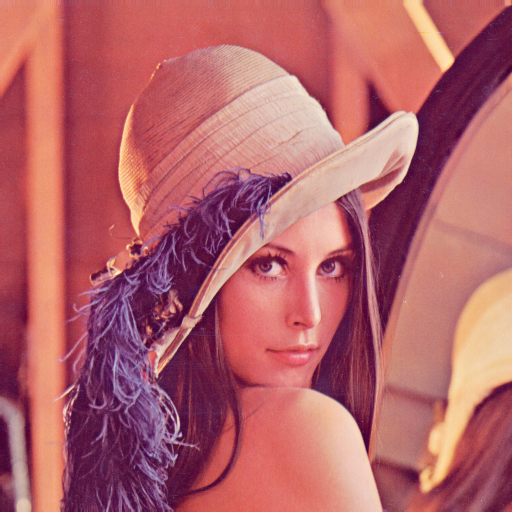
\includegraphics[scale=0.5]{Images/lena/lena_orig.png}
  \caption{Original Lena Image}
  \label{lena_o}
\end{figure}
Figure \ref{lena_o} is a standard test image for image processing and is good for our purposes since it contains a variety of different edges with different strengths.

So what we first do is define our convolution functions that we will be using in code.
\begin{lstlisting}
function combine_kernels(kers...)
    return reduce(conv2, kers)
end

function convolve_image(I, kers...)
    kernel = combine_kernels(kers...)
    return imfilter(I, centered(kernel))
end

function convolve_scale_space(L, kers...)
    return mapslices(
        scale_slice -> convolve_image(scale_slice, kers...),
        L,
        (1,2)
    )
end

function convolve_gaussian(img, sigma)
    # The dimension of the convolution matrix
    length = 8*ceil(Int, sigma) + 1
    return imfilter(img, reflect(Kernel.gaussian((sigma, sigma), (length, length))))
end
\end{lstlisting}
These will be used for computing all the neccessary two dimensional matrix convolutions that we will use throughout the rest of the code.
The next step is to then define our range of scales used and which derivative kernels we will be using to compute two dimensional discrete spatial derivatives.
The following code shows the definitions for our variables that will be used for all further calculations. 
\begin{lstlisting}
# Parameters
gamma = 1
scales = exp.(linspace(0, log(50), 40))

# Load the image
img = float.(ColorTypes.Gray.(testimage("lena_color_512")))

# Define derivative convolution matrices
Dy = Array(parent(Kernel.ando5()[1]))
Dx = Array(parent(Kernel.ando5()[2]))

# Normalized the derivatives
Dx /= sum(Dx .* (Dx .> 0))
Dy /= sum(Dy .* (Dy .> 0))
\end{lstlisting}
The derivative matrices used for our project are the ando5 matrices which are defined as the following
\begin{equation}
  \begin{aligned}
    [D_x] &=
    \begin{bmatrix}
      -0.003776 &-0.010199  &0.0  &0.010199  &0.003776 \\
      -0.026786 &-0.070844  &0.0  &0.070844  &0.026786 \\
      -0.046548 &-0.122572  &0.0  &0.122572  &0.046548 \\
      -0.026786 &-0.070844  &0.0  &0.070844  &0.026786 \\
      -0.003776 &-0.010199  &0.0  &0.010199  &0.003776
    \end{bmatrix} \\
    [D_y] &= [D_x]^T
  \end{aligned}
\end{equation}
From this point, we then can compute the scale space representation of our image and compute its spatial derivatives
The following section of code defines just how to do that.
\begin{lstlisting}
# Scale space representation
L = cat(3, (convolve_gaussian(img, sigma) for sigma in scales)...)

# First order derivatives
Lx = convolve_scale_space(L, Dx)
Ly = convolve_scale_space(L, Dy)

# Second order derivatives
Lxx = convolve_scale_space(Lx, Dx)
Lxy = convolve_scale_space(Lx, Dy)
Lyy = convolve_scale_space(Ly, Dy)

# Third order derivatives
Lxxx = convolve_scale_space(Lxx, Dx)
Lxxy = convolve_scale_space(Lxx, Dy)
Lxyy = convolve_scale_space(Lxy, Dy)
Lyyy = convolve_scale_space(Lyy, Dy)
\end{lstlisting}
By convolving our ando5 derivative matrix with the scale space representation, we can take spatial derivatives in both the $x$ and $y$ dimension. To give an idea of what the images look like, we have the following spatial derivatives of the image below.
% \begin{figure}[H]
%   \centering
%   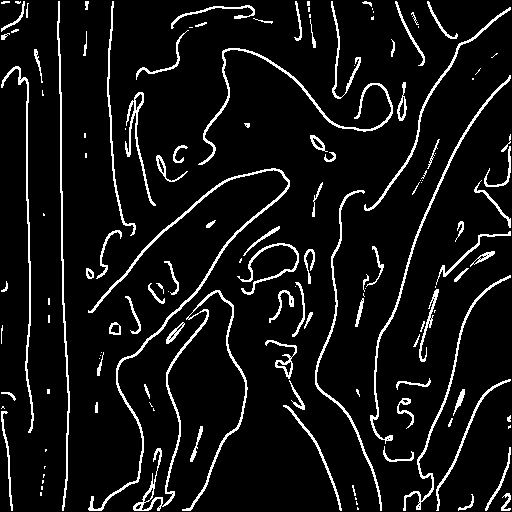
\includegraphics[scale=0.5]{{{Images/lena/lena_Lv_maxima_14.439}}}
%   \caption{Derivative of image in $x$ direction}
%   \label{lx}
% \end{figure}
% \begin{figure}[H]
%   \centering
%   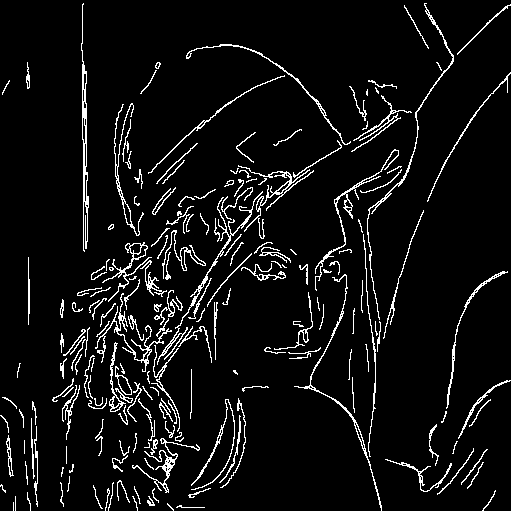
\includegraphics[scale=0.5]{Images/lena/lena_final.png}
%   \caption{Derivative of image in $y$ direction}
%   \label{ly}
% \end{figure}
Now that we have computed the spatial derivatives of the scale space representation of the image, we can check if we fulfill the conditions in (\ref{eq:c1}). 
The next step is to then calculate the edge strength derivatives neccessary to fulfill the conditions of (\ref{eq:c2}).
The code block below shows the computations for the edge strength based on the gradient magnitude and its derivatives.
\begin{lstlisting}
# Shape the scales vector to be a vector with depth
scales3 = reshape(scales, 1, 1, length(scales))

# Definition of the gradient edge strength (magnitude)
const GL = scales3.^(gamma).*(Lx.^2+Ly.^2)

# Derivative of edge strength gradinet with respect to scale
const GLt = @. gamma*scales3^(gamma-1)*(Lx^2 + Ly^2) + scales3^gamma*(Lx*(Lxxx + Lxyy) + Ly*(Lxxy + Lyyy))

# Second derivative of edge strength gradinet with respect to scale
const GLtt = @. (gamma*(gamma - 1)*scales3^(gamma - 2)*(Lx^2 + Ly^2) + 2gamma*scales3^(gamma-1)*(Lx*(Lxxx + Lxyy) + Ly*(Lxxy + Lyyy)) + scales3^gamma/2*((Lxxx + Lxyy)^2 + (Lxxy + Lyyy)^2 + Lx*(Lxxxxx + 2Lxxxyy + Lxyyyy) + Ly*(Lxxxxy + 2Lxxyyy + Lyyyyy))) < 0
\end{lstlisting}
With these calculations we now can check all the conditions necessary to define an edge in scale space. 


\begin{table}[H]
  \caption{Gradient magnitude}
  \centering
  \tabulinesep=0.1em
  \begin{tabu}to \textwidth{cX[c,m]X[c,m]X[c,m]}
    \toprule
    & Lena & Mandrill & Peppers\\
    \midrule
    $t = 0.1$ & 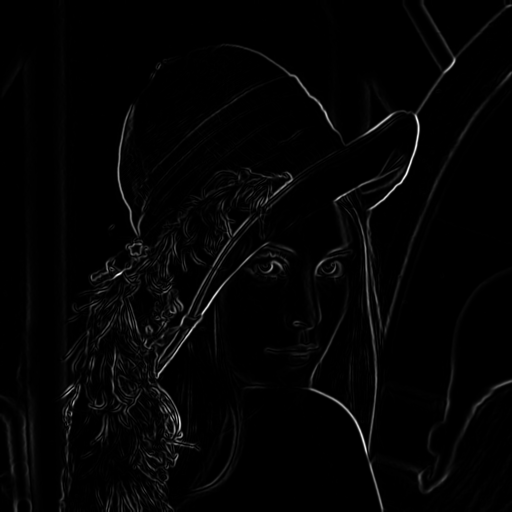
\includegraphics[height=11em]{{{Images/lena/lena_GL_0.1}}} & 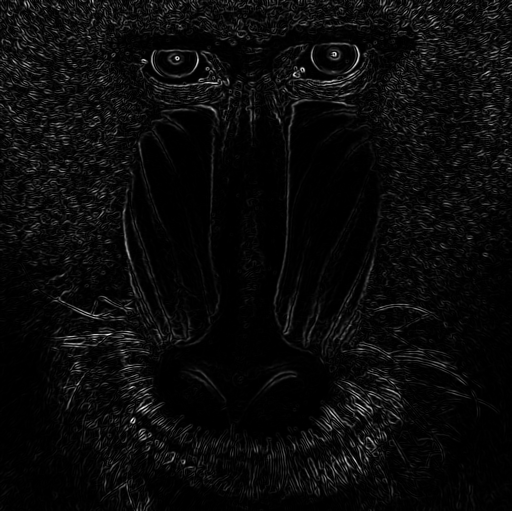
\includegraphics[height=11em]{{{Images/mandrill/mandrill_GL_0.1}}} &  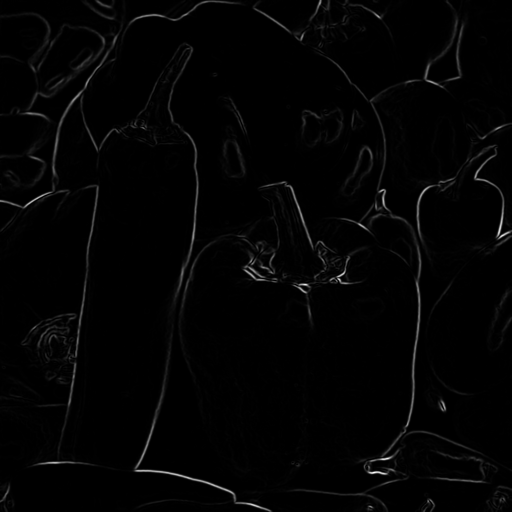
\includegraphics[height=11em]{{{Images/peppers/peppers_GL_0.1}}}\\
    $t = 1.7$ & 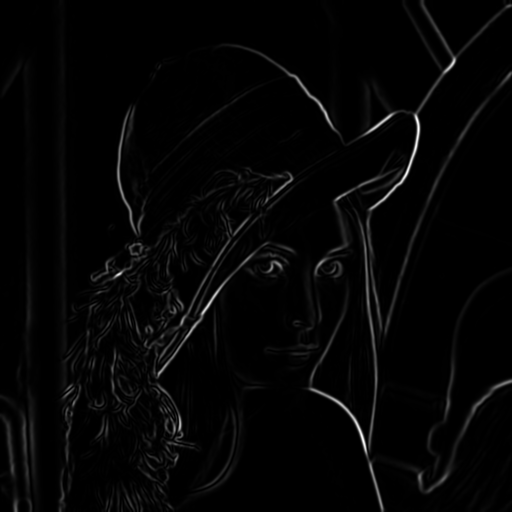
\includegraphics[height=11em]{{{Images/lena/lena_GL_1.7}}} & 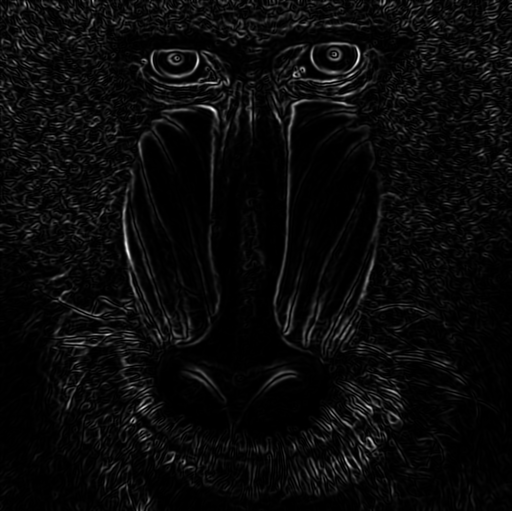
\includegraphics[height=11em]{{{Images/mandrill/mandrill_GL_1.7}}} & 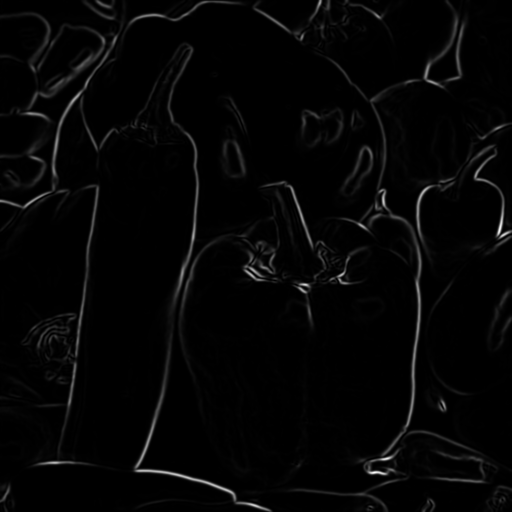
\includegraphics[height=11em]{{{Images/peppers/peppers_GL_1.7}}}\\
    $t = 18.7$ & 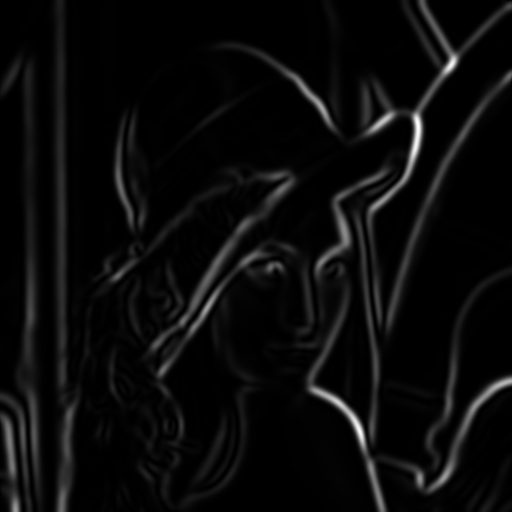
\includegraphics[height=11em]{{{Images/lena/lena_GL_18.7}}} & 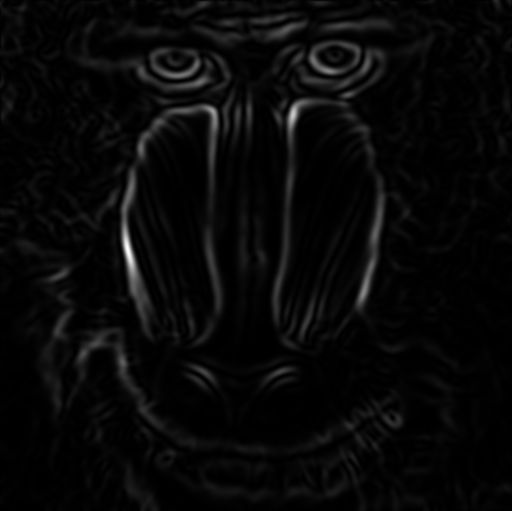
\includegraphics[height=11em]{{{Images/mandrill/mandrill_GL_18.7}}} &  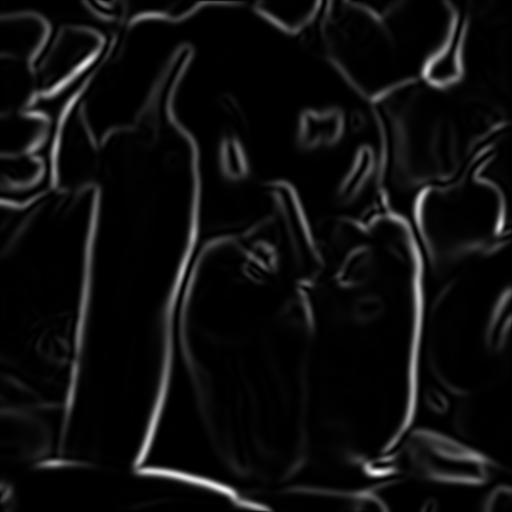
\includegraphics[height=11em]{{{Images/peppers/peppers_GL_18.7}}}\\
    $t = 93.6$ & 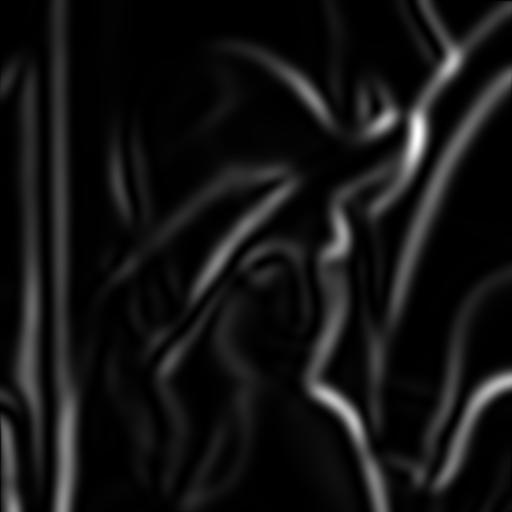
\includegraphics[height=11em]{{{Images/lena/lena_GL_93.6}}} & 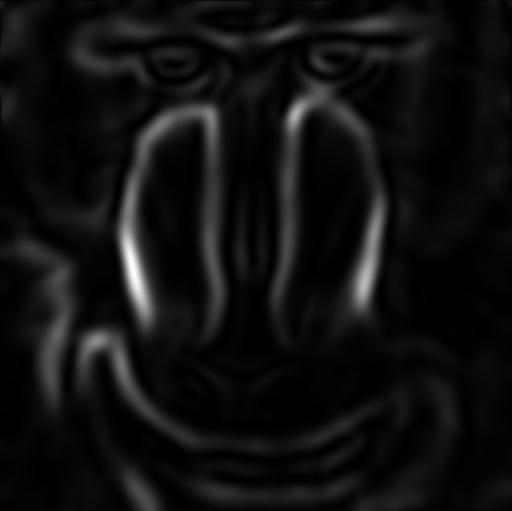
\includegraphics[height=11em]{{{Images/mandrill/mandrill_GL_93.6}}} &  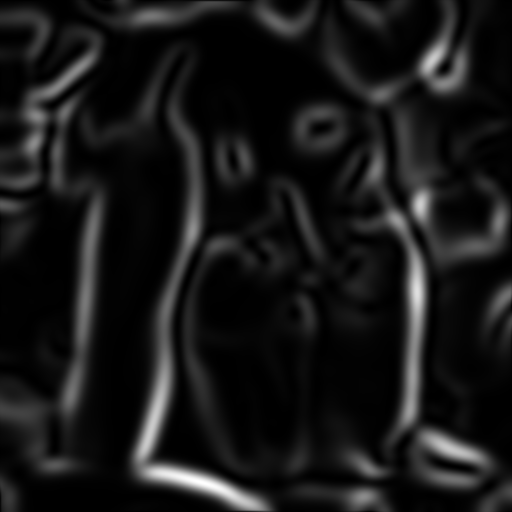
\includegraphics[height=11em]{{{Images/peppers/peppers_GL_93.6}}}\\
    $t = 256.0$ & 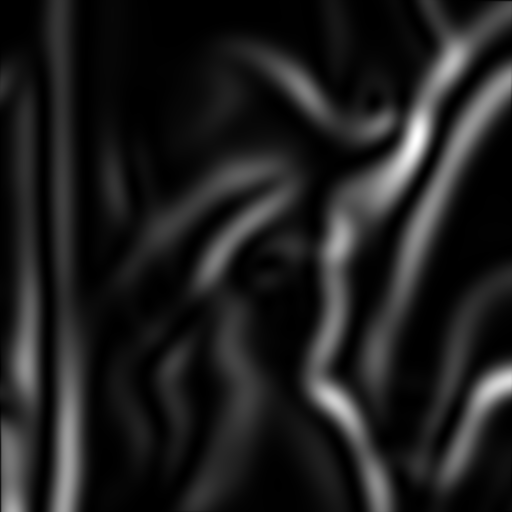
\includegraphics[height=11em]{{{Images/lena/lena_GL_256.0}}} & 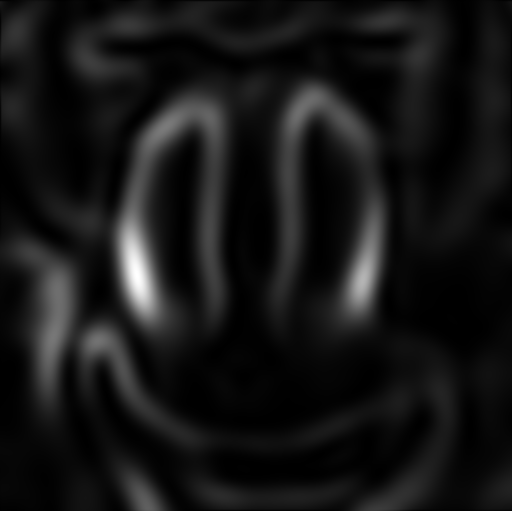
\includegraphics[height=11em]{{{Images/mandrill/mandrill_GL_256.0}}} &  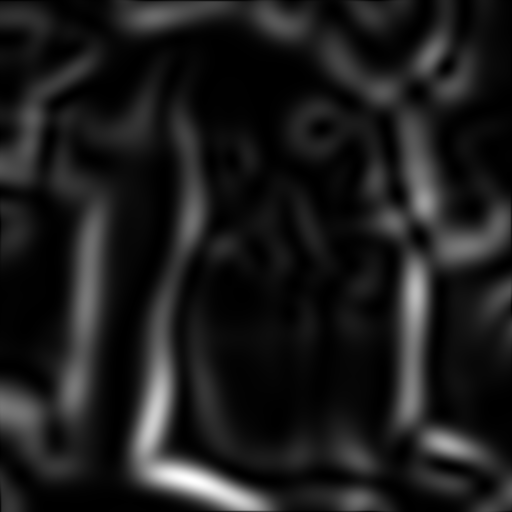
\includegraphics[height=11em]{{{Images/peppers/peppers_GL_256.0}}}\\
    \bottomrule
\end{tabu}
\end{table}
\begin{table}[H]
  \caption{First scale derivative of gradient magnitude}
  \centering
  \tabulinesep=0.1em
  \begin{tabu}to \textwidth{cX[c,m]X[c,m]X[c,m]}
    \toprule
    & Lena & Mandrill & Peppers\\
    \midrule
    $t = 0.1$ & 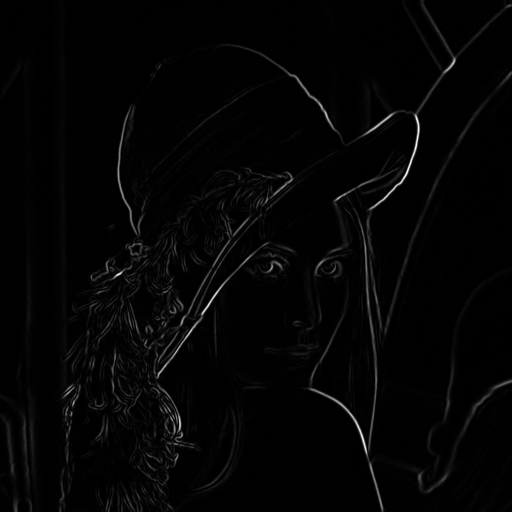
\includegraphics[height=11em]{{{Images/lena/lena_GLt_0.1}}} & 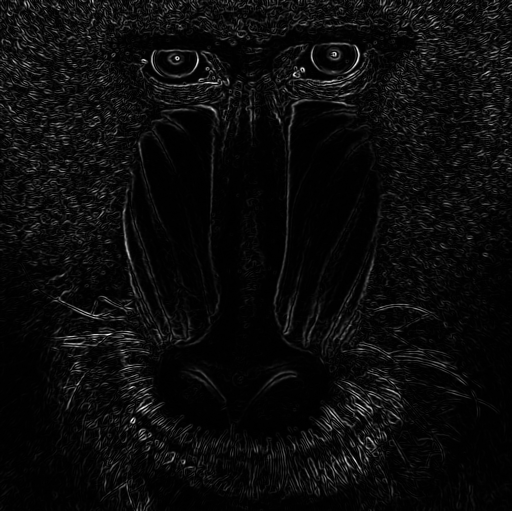
\includegraphics[height=11em]{{{Images/mandrill/mandrill_GLt_0.1}}} &  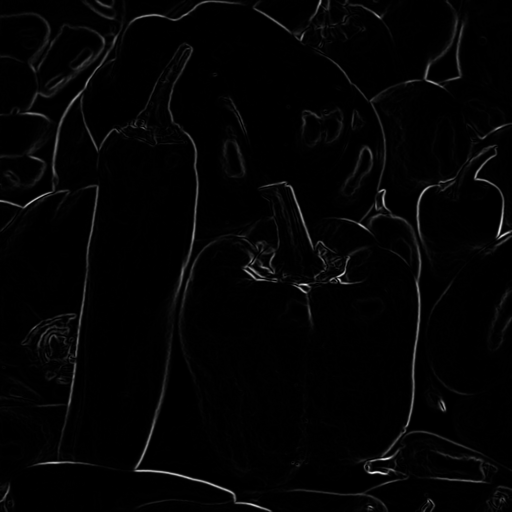
\includegraphics[height=11em]{{{Images/peppers/peppers_GLt_0.1}}}\\
    $t = 1.7$ & 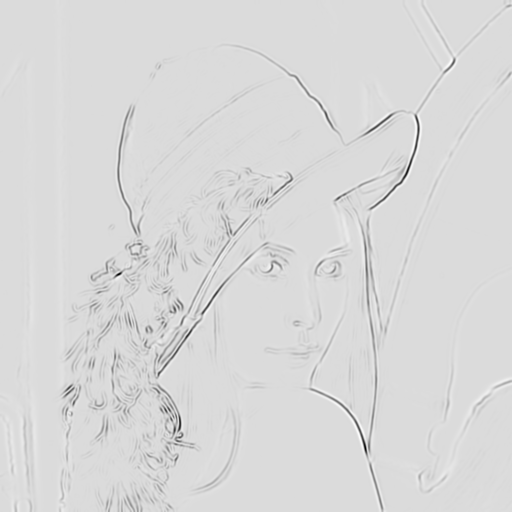
\includegraphics[height=11em]{{{Images/lena/lena_GLt_1.7}}} & 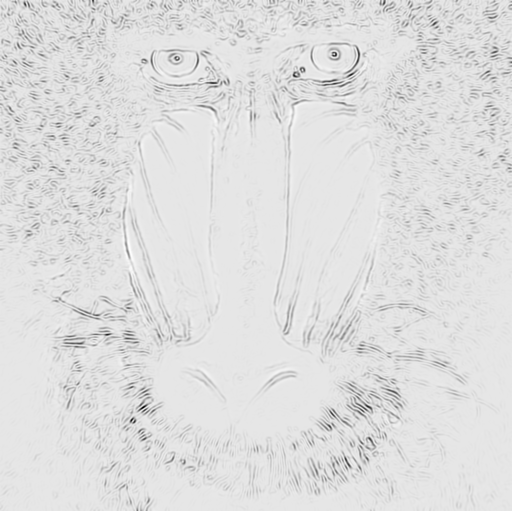
\includegraphics[height=11em]{{{Images/mandrill/mandrill_GLt_1.7}}} & 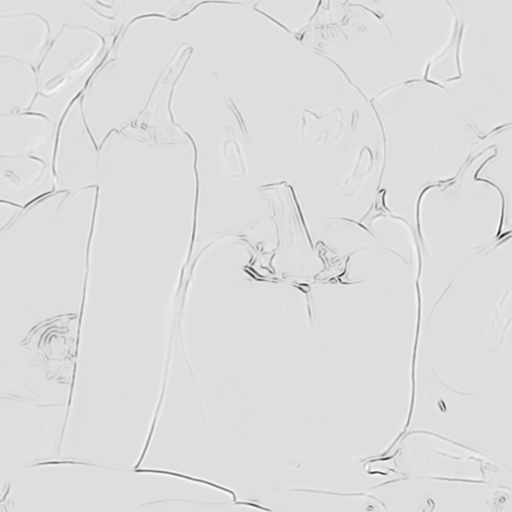
\includegraphics[height=11em]{{{Images/peppers/peppers_GLt_1.7}}}\\
    $t = 18.7$ & 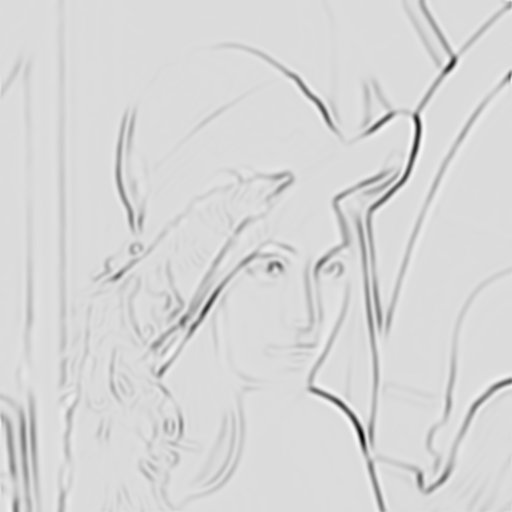
\includegraphics[height=11em]{{{Images/lena/lena_GLt_18.7}}} & 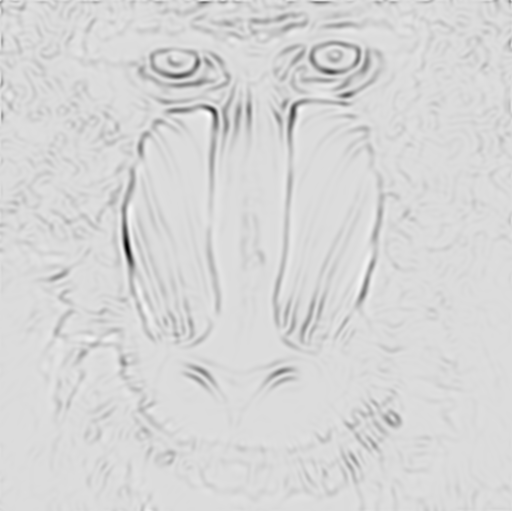
\includegraphics[height=11em]{{{Images/mandrill/mandrill_GLt_18.7}}} &  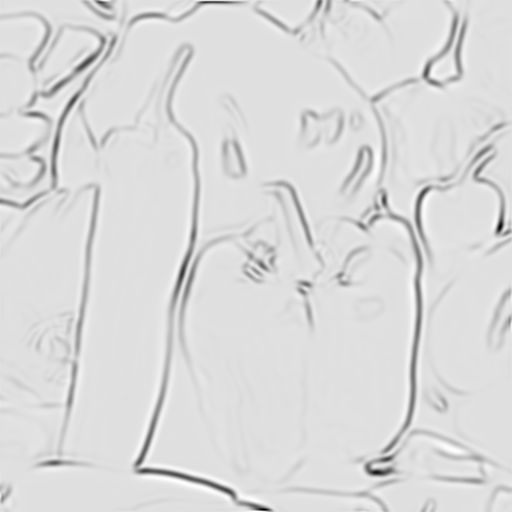
\includegraphics[height=11em]{{{Images/peppers/peppers_GLt_18.7}}}\\
    $t = 93.6$ & 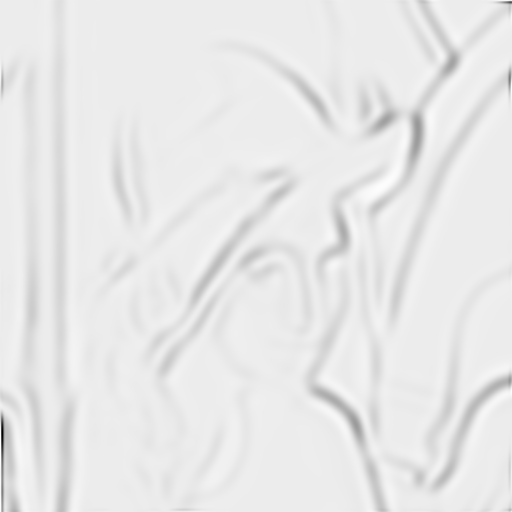
\includegraphics[height=11em]{{{Images/lena/lena_GLt_93.6}}} & 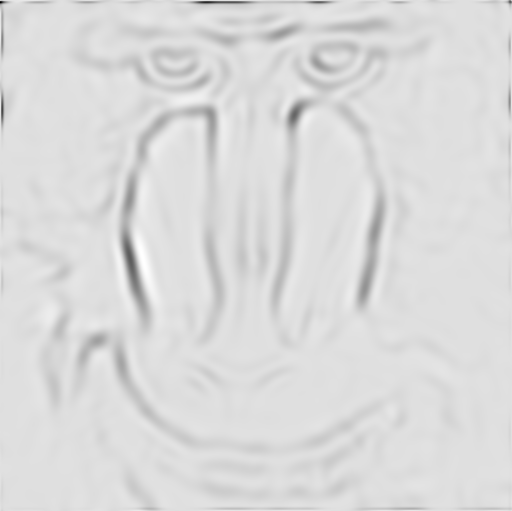
\includegraphics[height=11em]{{{Images/mandrill/mandrill_GLt_93.6}}} &  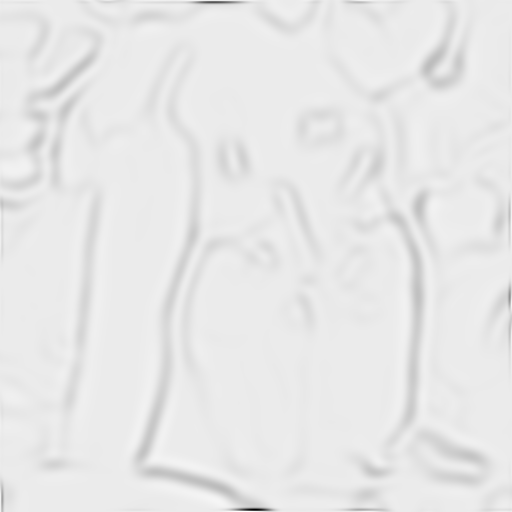
\includegraphics[height=11em]{{{Images/peppers/peppers_GLt_93.6}}}\\
    $t = 256.0$ & 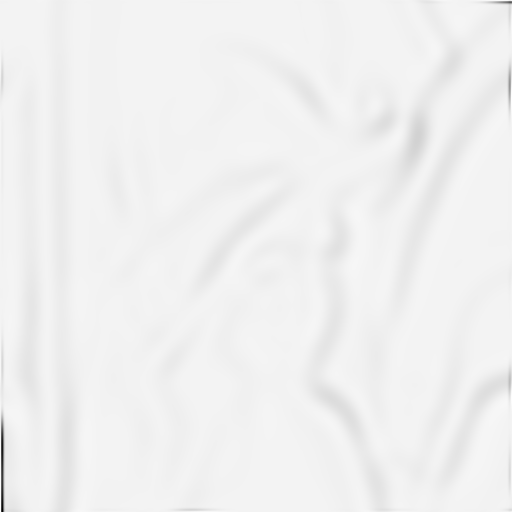
\includegraphics[height=11em]{{{Images/lena/lena_GLt_256.0}}} & 
\includegraphics[height=11em]{{{Images/mandrill/mandrill_GLt_256.0}}} &  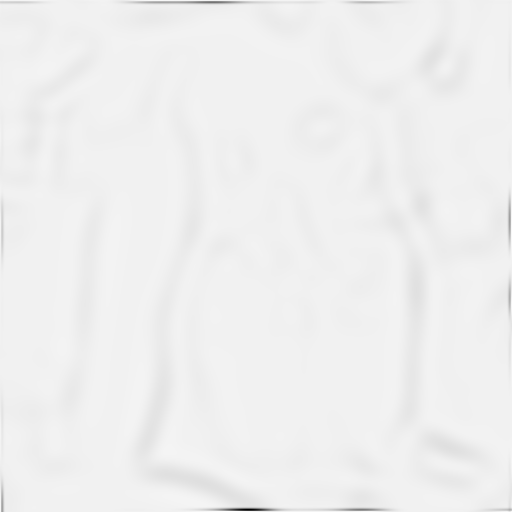
\includegraphics[height=11em]{{{Images/peppers/peppers_GLt_256.0}}}\\
    \bottomrule
\end{tabu}
\end{table}
\begin{table}[H]
  \caption{Second scale derivative of the gradient magnitude}
  \centering
  \tabulinesep=0.1em
  \begin{tabu}to \textwidth{cX[c,m]X[c,m]X[c,m]}
    \toprule
    & Lena & Mandrill & Peppers\\
    \midrule
    $t = 0.1$ & 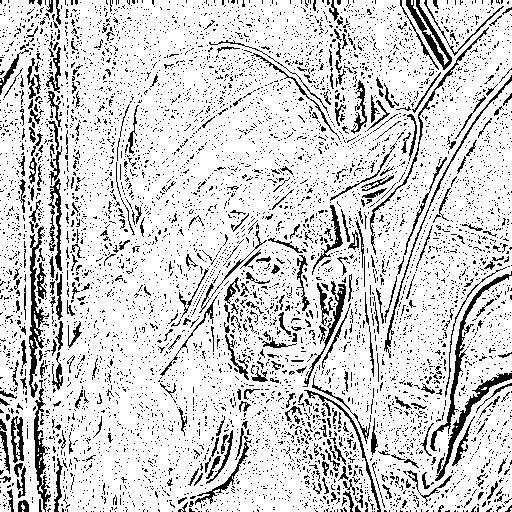
\includegraphics[height=11em]{{{Images/lena/lena_GLtt_0.1}}} & 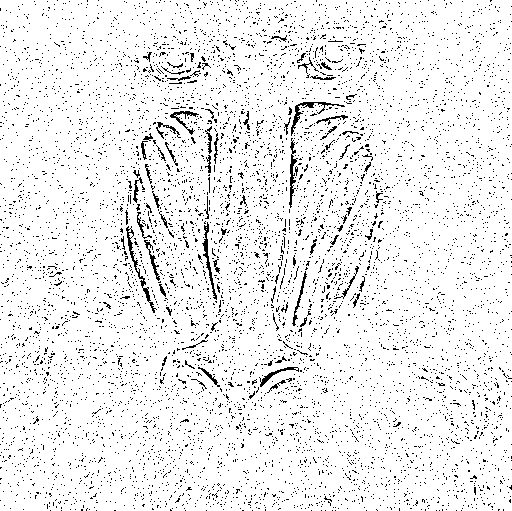
\includegraphics[height=11em]{{{Images/mandrill/mandrill_GLtt_0.1}}} &  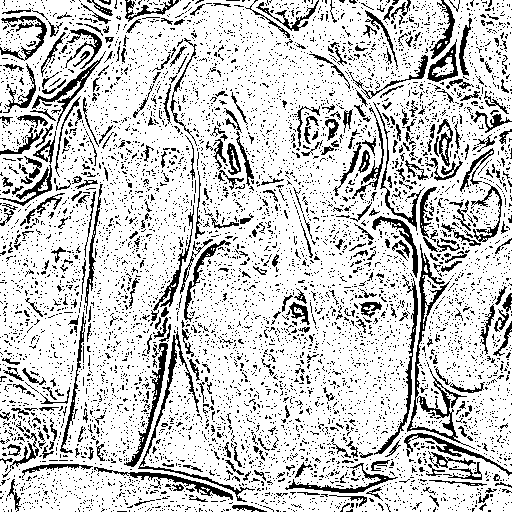
\includegraphics[height=11em]{{{Images/peppers/peppers_GLtt_0.1}}}\\
    $t = 1.7$ & 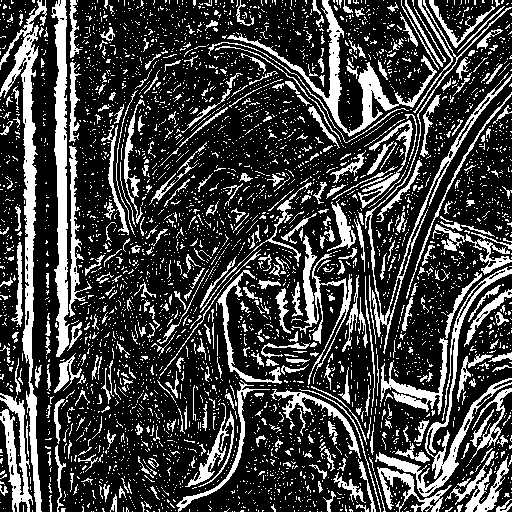
\includegraphics[height=11em]{{{Images/lena/lena_GLtt_1.7}}} & 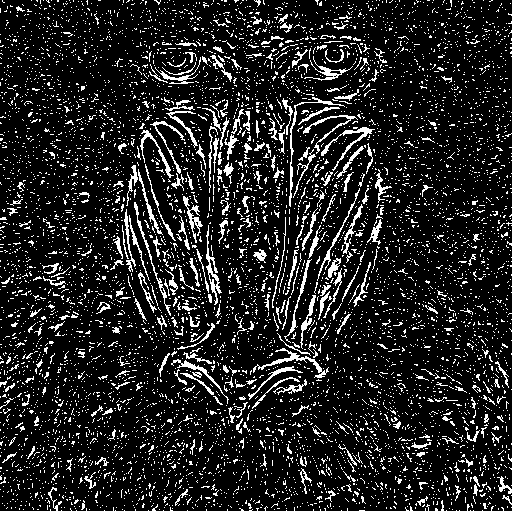
\includegraphics[height=11em]{{{Images/mandrill/mandrill_GLtt_1.7}}} & 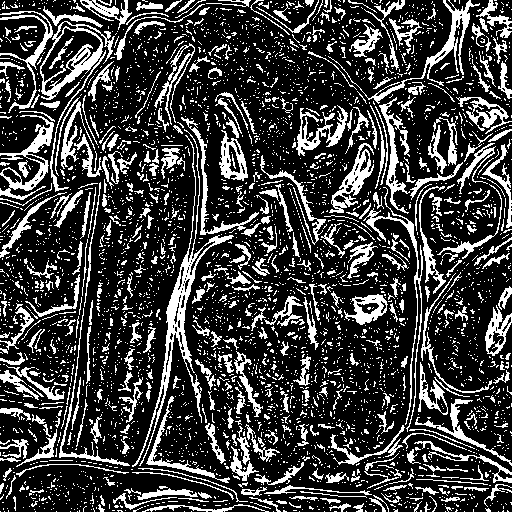
\includegraphics[height=11em]{{{Images/peppers/peppers_GLtt_1.7}}}\\
    $t = 18.7$ & 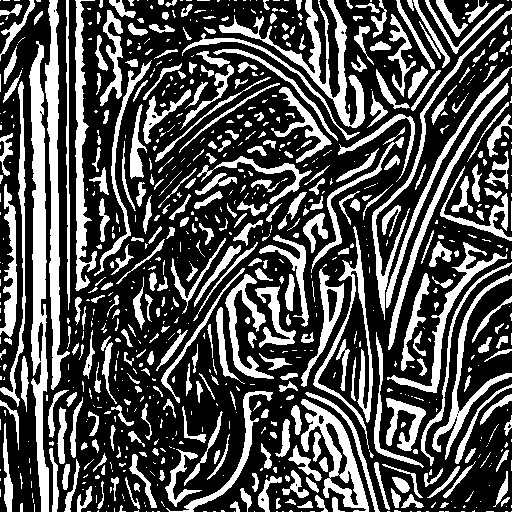
\includegraphics[height=11em]{{{Images/lena/lena_GLtt_18.7}}} & 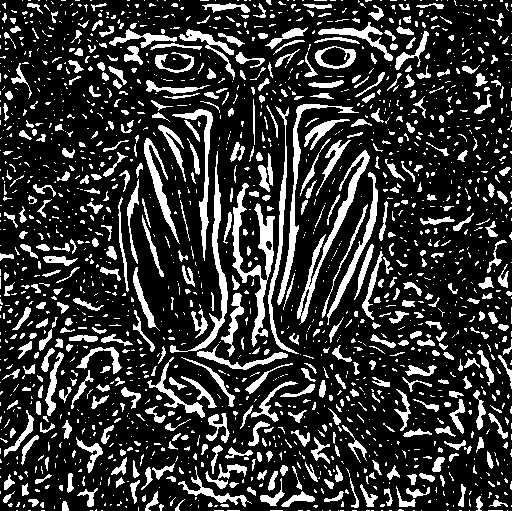
\includegraphics[height=11em]{{{Images/mandrill/mandrill_GLtt_18.7}}} &  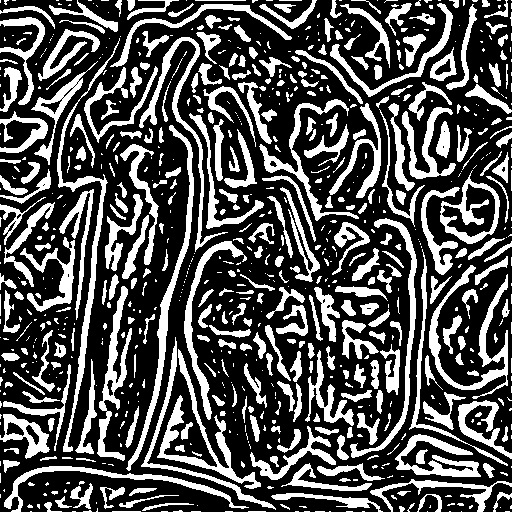
\includegraphics[height=11em]{{{Images/peppers/peppers_GLtt_18.7}}}\\
    $t = 93.6$ & 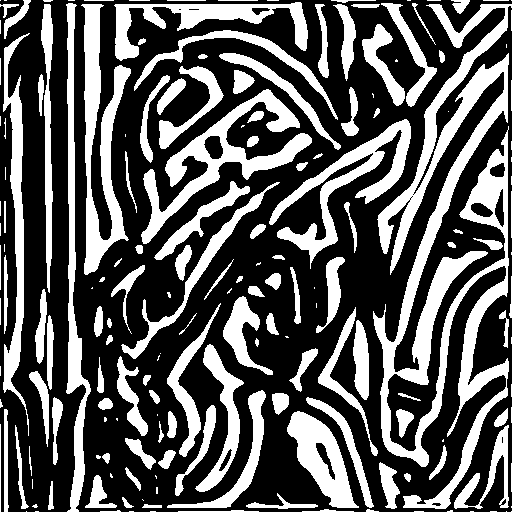
\includegraphics[height=11em]{{{Images/lena/lena_GLtt_93.6}}} & 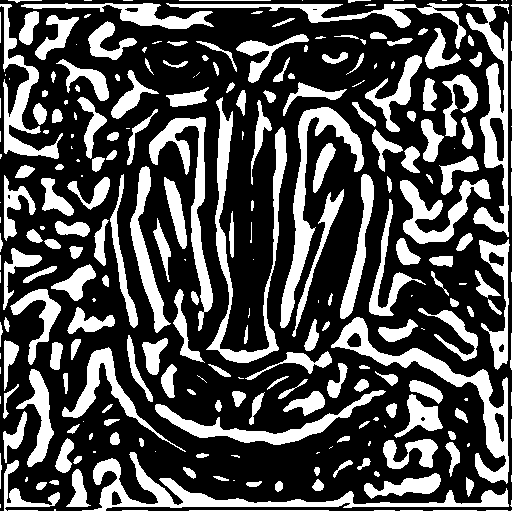
\includegraphics[height=11em]{{{Images/mandrill/mandrill_GLtt_93.6}}} &  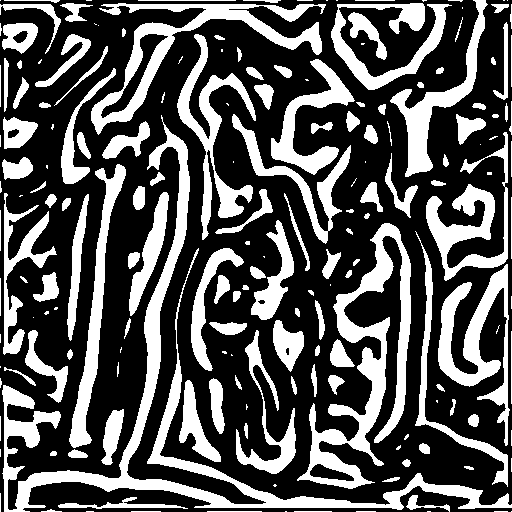
\includegraphics[height=11em]{{{Images/peppers/peppers_GLtt_93.6}}}\\
    $t = 256.0$ & 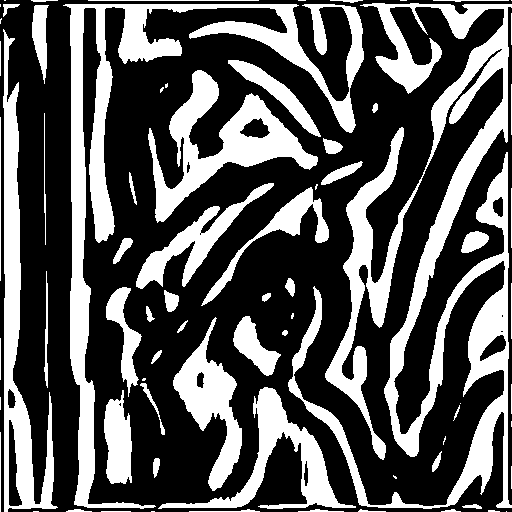
\includegraphics[height=11em]{{{Images/lena/lena_GLtt_256.0}}} & 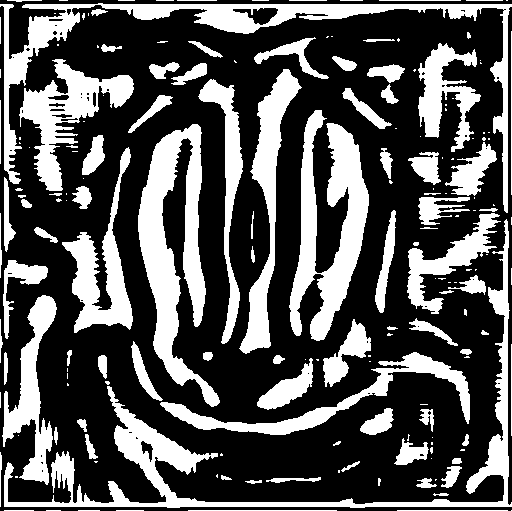
\includegraphics[height=11em]{{{Images/mandrill/mandrill_GLtt_256.0}}} &  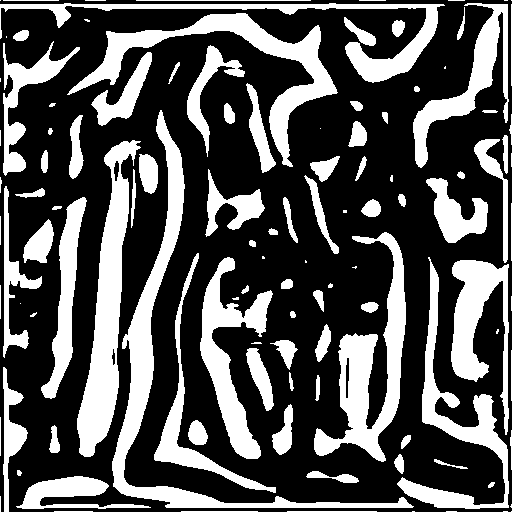
\includegraphics[height=11em]{{{Images/peppers/peppers_GLtt_256.0}}}\\
    \bottomrule
\end{tabu}
\end{table}
\begin{table}[H]
  \caption{Maxima of scale space in the $v$ direction}
  \centering
  \tabulinesep=0.1em
  \begin{tabu}to \textwidth{cX[c,m]X[c,m]X[c,m]}
    \toprule
    & Lena & Mandrill & Peppers\\
    \midrule
    $t = 0.1$ & 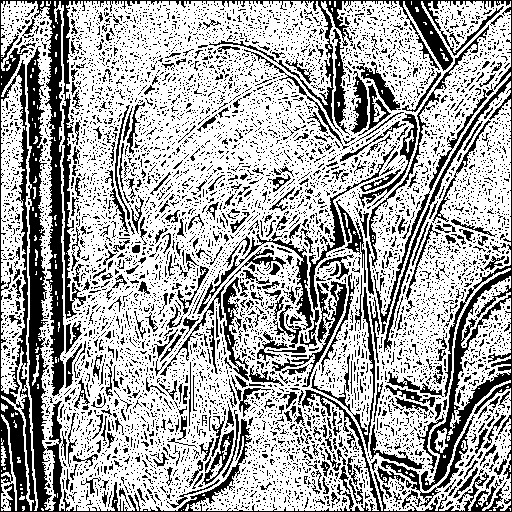
\includegraphics[height=11em]{{{Images/lena/lena_Lv_maxima_0.1}}} & 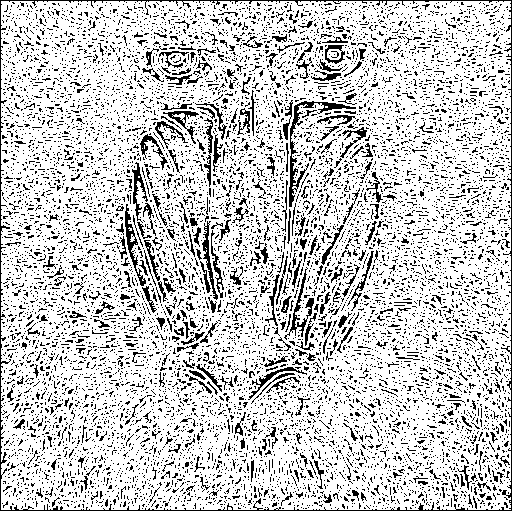
\includegraphics[height=11em]{{{Images/mandrill/mandrill_Lv_maxima_0.1}}} &  \includegraphics[height=11em]{{{Images/peppers/peppers_Lv_maxima_0.1}}}\\
    $t = 1.7$ & \includegraphics[height=11em]{{{Images/lena/lena_Lv_maxima_1.7}}} & \includegraphics[height=11em]{{{Images/mandrill/mandrill_Lv_maxima_1.7}}} & \includegraphics[height=11em]{{{Images/peppers/peppers_Lv_maxima_1.7}}}\\
    $t = 18.7$ & \includegraphics[height=11em]{{{Images/lena/lena_Lv_maxima_18.7}}} & \includegraphics[height=11em]{{{Images/mandrill/mandrill_Lv_maxima_18.7}}} &  \includegraphics[height=11em]{{{Images/peppers/peppers_Lv_maxima_18.7}}}\\
    $t = 93.6$ & \includegraphics[height=11em]{{{Images/lena/lena_Lv_maxima_93.6}}} & \includegraphics[height=11em]{{{Images/mandrill/mandrill_Lv_maxima_93.6}}} &  \includegraphics[height=11em]{{{Images/peppers/peppers_Lv_maxima_93.6}}}\\
    $t = 256.0$ & \includegraphics[height=11em]{{{Images/lena/lena_Lv_maxima_256.0}}} & \includegraphics[height=11em]{{{Images/mandrill/mandrill_Lv_maxima_256.0}}} &  \includegraphics[height=11em]{{{Images/peppers/peppers_Lv_maxima_256.0}}}\\
    \bottomrule
\end{tabu}
\end{table}
\begin{table}[H]
  \caption{The second derivative of the scale space with respect to the $v$ direction}
  \centering
  \tabulinesep=0.1em
  \begin{tabu}to \textwidth{cX[c,m]X[c,m]X[c,m]}
    \toprule
    & Lena & Mandrill & Peppers\\
    \midrule
    $t = 0.1$ & \includegraphics[height=11em]{{{Images/lena/lena_Lvv_0.1}}} & \includegraphics[height=11em]{{{Images/mandrill/mandrill_Lvv_0.1}}} &  \includegraphics[height=11em]{{{Images/peppers/peppers_Lvv_0.1}}}\\
    $t = 1.7$ & \includegraphics[height=11em]{{{Images/lena/lena_Lvv_1.7}}} & \includegraphics[height=11em]{{{Images/mandrill/mandrill_Lvv_1.7}}} & \includegraphics[height=11em]{{{Images/peppers/peppers_Lvv_1.7}}}\\
    $t = 18.7$ & \includegraphics[height=11em]{{{Images/lena/lena_Lvv_18.7}}} & \includegraphics[height=11em]{{{Images/mandrill/mandrill_Lvv_18.7}}} &  \includegraphics[height=11em]{{{Images/peppers/peppers_Lvv_18.7}}}\\
    $t = 93.6$ & \includegraphics[height=11em]{{{Images/lena/lena_Lvv_93.6}}} & \includegraphics[height=11em]{{{Images/mandrill/mandrill_Lvv_93.6}}} &  \includegraphics[height=11em]{{{Images/peppers/peppers_Lvv_93.6}}}\\
    $t = 256.0$ & \includegraphics[height=11em]{{{Images/lena/lena_Lvv_256.0}}} & \includegraphics[height=11em]{{{Images/mandrill/mandrill_Lvv_256.0}}} &  \includegraphics[height=11em]{{{Images/peppers/peppers_Lvv_256.0}}}\\
    \bottomrule
\end{tabu}
\end{table}
\begin{table}[H]
  \caption{The third derivative of the scale space with respect to the $v$ direction}
  \centering
  \tabulinesep=0.1em
  \begin{tabu}to \textwidth{cX[c,m]X[c,m]X[c,m]}
    \toprule
    & Lena & Mandrill & Peppers\\
    \midrule
    $t = 0.1$ & \includegraphics[height=11em]{{{Images/lena/lena_Lvvv_0.1}}} & \includegraphics[height=11em]{{{Images/mandrill/mandrill_Lvvv_0.1}}} &  \includegraphics[height=11em]{{{Images/peppers/peppers_Lvvv_0.1}}}\\
    $t = 1.7$ & \includegraphics[height=11em]{{{Images/lena/lena_Lvvv_1.7}}} & \includegraphics[height=11em]{{{Images/mandrill/mandrill_Lvvv_1.7}}} & \includegraphics[height=11em]{{{Images/peppers/peppers_Lvvv_1.7}}}\\
    $t = 18.7$ & \includegraphics[height=11em]{{{Images/lena/lena_Lvvv_18.7}}} & \includegraphics[height=11em]{{{Images/mandrill/mandrill_Lvvv_18.7}}} &  \includegraphics[height=11em]{{{Images/peppers/peppers_Lvvv_18.7}}}\\
    $t = 93.6$ & \includegraphics[height=11em]{{{Images/lena/lena_Lvvv_93.6}}} & \includegraphics[height=11em]{{{Images/mandrill/mandrill_Lvvv_93.6}}} &  \includegraphics[height=11em]{{{Images/peppers/peppers_Lvvv_93.6}}}\\
    $t = 256.0$ & \includegraphics[height=11em]{{{Images/lena/lena_Lvvv_256.0}}} & \includegraphics[height=11em]{{{Images/mandrill/mandrill_Lvvv_256.0}}} &  \includegraphics[height=11em]{{{Images/peppers/peppers_Lvvv_256.0}}}\\
    \bottomrule
\end{tabu}
\end{table}

\subsection{Marching Cubes}

We note that the equations $\partial_t (\mathcal G_{\text{$\gamma$-norm}} L) =0 $ and $L_{vv} = 0$ define isosurfaces $\mathcal Z_1$ and $\mathcal Z_2$, embedded in $L$.
Computing the intersection of these two surfaces and requiring the local maxima conditions $\partial_{tt} (\mathcal G_{\text{$\gamma$-norm}} L) < 0$ and $L_{vvv} < 0$ yields a family of isocurves, also embedded in $L$, which directly correspond to the edges in the image.

However, since we only have access to $\partial_t (\mathcal G_{\text{$\gamma$-norm}} L)$ and $L_{vv}$ at the lattice points of $L$, we cannot solve for their intersection analytically.
Instead, we rely on an approximation method to find the edges.
We have chosen to implement the algorithm sketched by Lindeberg, a variation of the marching cubes algorithm.

In our implementation, $L$ is broken down into voxels with a value at every corner.
\begin{lstlisting}
function marching_cubes(x, y, t, visited)
    if visited[x, y, t]
        return Set()
    end

    visited[x, y, t] = true
\end{lstlisting}
Since edges are connected sets of points, we know that if a given voxel has already been visited it cannot be part of this edge, so we skip it.

\begin{lstlisting}
    const corners = (x:x+1, y:y+1, t:t+1)

    # Note: Maybe they don't need to be in the same corner
    if !(any(view(GLtt, corners...)) && any(view(Lvvv, corners...)))
      return Set()
    end
\end{lstlisting}
We then check that our sign conditions $\mathcal S_1 < 0$ and $\mathcal S_2 < 0$ are each negative in at least one vertex of the voxel, otherwise there can be no maxima of $\mathcal Z_1$ and $\mathcal Z_2$ inside this voxel.
\begin{lstlisting}
    @views Z1, Z2 = Lvv[corners...], GLt[corners...]
    Z1_crossings = Array{Tuple{NTuple{3,Int}, NTuple{3,Int}, Array{Float64, 1}}, 1}()
    Z2_crossings = Array{Tuple{NTuple{3,Int}, NTuple{3,Int}, Array{Float64, 1}}, 1}()

    # Find all sign crossings w/ linear interpolation
    for (a, b) in cube_edges
        if signbit(Z1[a...]) != signbit(Z1[b...])
            push!(Z1_crossings, (a, b, linear_interpolate(a, b, Z1[a...], Z1[b...])))
        end

        if signbit(Z2[a...]) != signbit(Z2[b...])
            push!(Z2_crossings, (a, b, linear_interpolate(a, b, Z2[a...], Z2[b...])))
        end
    end
\end{lstlisting}

We then construct a list of edges where the signs of $\mathcal Z_1$ or $\mathcal Z_2$ differ at the endpoints of the edge.
We then estimate the position of the zero crossing of the surface of that point using linear interpolation.
\begin{lstlisting}
    for (normal, face) in cube_faces
        Z1_zeros, Z2_zeros = [], []
        for (a, b, mid) in Z1_crossings
            if a in face && b in face
                push!(Z1_zeros, mid)
            end
        end

        for (a, b, mid) in Z2_crossings
            if a in face && b in face
                push!(Z2_zeros, mid)
            end
        end
\end{lstlisting}
Then, for every face of the voxel, we collect all of the edges with a zero crossing that lie on that face.
\begin{lstlisting}
        # Reject if there are more than two crossings for either invariant
        if !(length(Z1_zeros) == length(Z2_zeros) == 2)
            continue
        end
\end{lstlisting}
If there is only one edge with a zero crossing on that face, the face cannot have a zero crossing inside it, so we skip further processing on this face.
If there are four zero crossings of either invariant on this face, then it is ambiguous how the isosurface intersects with the face, so we will skip it\footnote{In the future, we could try to resolve this situation, since there are only two possible cases.} Here is a visualization of one case satisfying these requirements:

\tdplotsetmaincoords{70}{120}
\begin{center}
  \begin{tabu}{cc}
    \toprule
    $\mathcal Z_1 $(i.e. $L_{vv}$)& $\mathcal Z_2$ (i.e. $\mathcal{G}L_t$)\\
    \midrule
    \begin{tikzpicture}[scale=0.5,tdplot_main_coords]
      % The vertex at V
      \tdplotsetcoord{P}{sqrt(3)*5}{55}{45}
      \tdplotsetcoord{O}{0}{0}{0}

      \draw[]
      (0,0,0) -- (Px)
      (0,0,0) -- (Py)
      (0,0,0) -- (Pz);

      \draw[] (Pxz) -- (P) -- (Pxy) -- (Px) -- (Pxz) -- (Pz) -- (Pyz) -- (P);
      \draw[] (Pyz) -- (Py) -- (Pxy);

      \node[fill,circle,inner sep=1.75pt] at ($ (P)!0.63!(Pyz) $) {};
      \node[fill,circle,inner sep=1.75pt] at ($ (Pxy)!0.45!(Py) $) {};
      \draw [thick] ($ (P)!0.63!(Pyz) $)--($ (Pxy)!0.45!(Py) $);

      \node[fill,circle,inner sep=1.75pt] at ($ (Pxz)!0.4!(Pz) $) {};
      \node[fill,circle,inner sep=1.75pt] at ($ (Px)!0.75!(O) $) {};
      \draw [thick] ($ (Pxz)!0.4!(Pz) $)--($ (Px)!0.75!(O) $);

      \node[label=above:$+$,fill,circle,inner sep=1.3pt] at (P) {};
      \node[label=below left:$+$,fill,circle,inner sep=1.3pt] at (Px) {};
      \node[label=below right:$-$,fill,circle,inner sep=1.3pt] at (Py) {};
      \node[label=above:$-$,fill,circle,inner sep=1.3pt] at (Pz) {};
      \node[label=below:$+$,fill,circle,inner sep=1.3pt] at (Pxy) {};
      \node[label=above right:$-$,fill,circle,inner sep=1.3pt] at (Pyz) {};
      \node[label=above left:$+$,fill,circle,inner sep=1.3pt] at (Pxz) {};
      \node[label=above right:$-$,fill,circle,inner sep=1.3pt] at (O) {};
    \end{tikzpicture} &
    \begin{tikzpicture}[scale=0.5,tdplot_main_coords]
      % The vertex at V
      \tdplotsetcoord{P}{sqrt(3)*5}{55}{45}
      \tdplotsetcoord{O}{0}{0}{0}

      \draw[]
      (0,0,0) -- (Px)
      (0,0,0) -- (Py)
      (0,0,0) -- (Pz);

      \draw[]
      (Pxz) -- (P) -- (Pxy) -- (Px) -- (Pxz) -- (Pz) -- (Pyz) -- (P);
      \draw[]
      (Pyz) -- (Py) -- (Pxy);

      \node[fill,circle,inner sep=1.75pt] at ($ (Px)!0.63!(Pxz) $) {};
      \node[fill,circle,inner sep=1.75pt] at ($ (O)!0.3!(Pz) $) {};
      \draw [thick] ($ (Px)!0.63!(Pxz) $)--($ (O)!0.3!(Pz) $);

      \node[fill,circle,inner sep=1.75pt] at ($ (Pxy)!0.7!(P) $) {};
      \node[fill,circle,inner sep=1.75pt] at ($ (Py)!0.3!(Pyz) $) {};

      \draw [thick] ($ (Pxy)!0.7!(P) $)--($ (Py)!0.3!(Pyz) $);

      \node[label=above:$+$,fill,circle,inner sep=1.3pt] at (P) {};
      \node[label=below left:$-$,fill,circle,inner sep=1.3pt] at (Px) {};
      \node[label=below right:$-$,fill,circle,inner sep=1.3pt] at (Py) {};
      \node[label=above:$+$,fill,circle,inner sep=1.3pt] at (Pz) {};
      \node[label=below:$-$,fill,circle,inner sep=1.3pt] at (Pxy) {};
      \node[label=above right:$+$,fill,circle,inner sep=1.3pt] at (Pyz) {};
      \node[label=above left:$+$,fill,circle,inner sep=1.3pt] at (Pxz) {};
      \node[label=above right:$-$,fill,circle,inner sep=1.3pt] at (O) {};
    \end{tikzpicture}\\
    \bottomrule
  \end{tabu}
\end{center}
We then continue our processing:
\begin{lstlisting}
        # Check that the intersection lies on a face
        distance, midpoint = get(intersect)
        if distance > epsilon || !all(1 - epsilon .<= midpoint .<= 2 + epsilon)
            continue
        end

        push!(face_intersections, normal)
\end{lstlisting}
We check whether or not the lines caused by connecting the estimated zero crossings of the edges on the face intersect.
If they do, we mark that face as featuring an intersection, as shown here:
\begin{center}
  \begin{tikzpicture}[scale=0.5,tdplot_main_coords]
    % The vertex at V
    \tdplotsetcoord{P}{sqrt(3)*5}{55}{45}
    \tdplotsetcoord{O}{0}{0}{0}

    \draw[]
    (0,0,0) -- (Px)
    (0,0,0) -- (Py)
    (0,0,0) -- (Pz);

    \draw[]
    (Pxz) -- (P) -- (Pxy) -- (Px) -- (Pxz) -- (Pz) -- (Pyz) -- (P);
    \draw[]
    (Pyz) -- (Py) -- (Pxy);

    \draw[fill,fill opacity=0.15] (P) -- (Pyz) -- (Py) -- (Pxy);
    \draw[fill,fill opacity=0.15] (O) -- (Pz) -- (Pxz) -- (Px);

    \draw [thick, name path=face1a] ($ (Px)!0.63!(Pxz) $)--($ (O)!0.3!(Pz) $);
    \draw [thick, name path=face1b] ($ (Pxz)!0.4!(Pz) $)--($ (Px)!0.75!(O) $);

    \draw [thick, name path=face2a] ($ (Pxy)!0.7!(P) $)--($ (Py)!0.3!(Pyz) $);
    \draw [thick, name path=face2b] ($ (P)!0.63!(Pyz) $)--($ (Pxy)!0.45!(Py) $);

    \path [name intersections={of=face1a and face1b,by=F1}];
    \path [name intersections={of=face2a and face2b,by=F2}];

    \node[fill,circle,inner sep=1.7pt] at (F1) {};
    \node[fill,circle,inner sep=1.7pt] at (F2) {};
  \end{tikzpicture}
\end{center}
Continuing our processing:
\begin{lstlisting}
    if length(face_intersections) == 2
        for normal in face_intersections
            next_voxel = [x, y, t] + normal
            if all(1 .<= next_voxel .<= size(visited))
                union!(result, marching_cubes(next_voxel..., visited))
            end
        end
        push!(result, (x, y, t))
    end
\end{lstlisting}
If there are exactly two faces with zero crossings, then the voxel contains an edge segment.
We then extend the line defined by connecting the estimated intersection points on each face into the neighboring voxels:
\begin{center}
  \begin{tikzpicture}[scale=0.5,tdplot_main_coords]
    % The vertex at V
    \tdplotsetcoord{P}{sqrt(3)*5}{55}{45}
    \tdplotsetcoord{O}{0}{0}{0}

    \draw[]
    (0,0,0) -- (Px)
    (0,0,0) -- (Py)
    (0,0,0) -- (Pz);

    \draw[]
    (Pxz) -- (P) -- (Pxy) -- (Px) -- (Pxz) -- (Pz) -- (Pyz) -- (P);
    \draw[]
    (Pyz) -- (Py) -- (Pxy);

    \draw[transform canvas={shift={(Py)}}]
    (0,0,0) -- (Px)
    (0,0,0) -- (Py)
    (0,0,0) -- (Pz);
    \draw[transform canvas={shift={(Py)}}]
    (Pxz) -- (P) -- (Pxy) -- (Px) -- (Pxz) -- (Pz) -- (Pyz) -- (P);
    \draw[transform canvas={shift={(Py)}}]
    (Pyz) -- (Py) -- (Pxy);

    \draw[transform canvas={shift={($(0,0,0) - (Py)$)}}]
    (0,0,0) -- (Px)
    (0,0,0) -- (Py)
    (0,0,0) -- (Pz);
    \draw[transform canvas={shift={($(0,0,0) - (Py)$)}}]
    (Pxz) -- (P) -- (Pxy) -- (Px) -- (Pxz) -- (Pz) -- (Pyz) -- (P);
    \draw[transform canvas={shift={($(0,0,0) - (Py)$)}}]
    (Pyz) -- (Py) -- (Pxy);

    \draw[fill,fill opacity=0.15] (P) -- (Pyz) -- (Py) -- (Pxy);
    \draw[fill,fill opacity=0.15] (O) -- (Pz) -- (Pxz) -- (Px);

    \draw [dashed, name path=face1a] ($ (Px)!0.63!(Pxz) $)--($ (O)!0.3!(Pz) $);
    \draw [dashed, name path=face1b] ($ (Pxz)!0.4!(Pz) $)--($ (Px)!0.75!(O) $);

    \draw [dashed, name path=face2a] ($ (Pxy)!0.7!(P) $)--($ (Py)!0.3!(Pyz) $);
    \draw [dashed, name path=face2b] ($ (P)!0.63!(Pyz) $)--($ (Pxy)!0.45!(Py) $);

    \path [name intersections={of=face1a and face1b,by=F1}];
    \path [name intersections={of=face2a and face2b,by=F2}];

    \draw [thick, <->] ($(F1)!-0.5!(F2)$) -- ($(F1)!1.5!(F2)$);

    \node[fill,circle,inner sep=1.7pt] at (F1) {};
    \node[fill,circle,inner sep=1.7pt] at (F2) {};

  \end{tikzpicture}
\end{center}
The process is then repeated on the neighboring voxels until we have traversed the entire edge connected to this point.


% \begin{tikzpicture}[tdplot_main_coords]
%   % The vertex at V
%   \tdplotsetcoord{P}{sqrt(3)*5}{55}{45}
%   \tdplotsetcoord{O}{0}{0}{0}

%   \draw[thick]
%   (0,0,0) -- (Px)
%   (0,0,0) -- (Py)
%   (0,0,0) -- (Pz);

%   \draw[thick]
%   (Pxz) -- (P) -- (Pxy) -- (Px) -- (Pxz) -- (Pz) -- (Pyz) -- (P);
%   \draw[thick]
%   (Pyz) -- (Py) -- (Pxy);

%   \node[label=above:$P$,fill,circle,inner sep=1.75pt] at (P) {};
%   \node[label=below left:$Px$,fill,circle,inner sep=1.75pt] at (Px) {};
%   \node[label=below right:$Py$,fill,circle,inner sep=1.75pt] at (Py) {};
%   \node[label=above:$Pz$,fill,circle,inner sep=1.75pt] at (Pz) {};
%   \node[label=below:$Pxy$,fill,circle,inner sep=1.75pt] at (Pxy) {};
%   \node[label=above right:$Pyz$,fill,circle,inner sep=1.75pt] at (Pyz) {};
%   \node[label=above left:$Pxz$,fill,circle,inner sep=1.75pt] at (Pxz) {};
%   \node[label=above right:$O$,fill,circle,inner sep=1.75pt] at (O) {};
% \end{tikzpicture}
\section*{Appendix}

% \lstinputlisting[caption={edge\_detect.jl},label=edge_detect,frame=none]{edge_detect.jl}

\section*{References}

\end{document}
